% Build the vectors with the project Python: python report_figures.py
% Compile from this directory with pdflatex -jobname=RenalLens_Report main.tex.
\documentclass[10pt,a4paper]{article}
\usepackage[T1]{fontenc}
\usepackage[utf8]{inputenc}
\usepackage[english]{babel}
\usepackage{lmodern,charter,microtype}
\usepackage{graphicx,xcolor,booktabs,hyperref,fancyhdr}
\usepackage[a4paper,left=19mm,right=19mm,top=15mm,bottom=17mm,footskip=9mm]{geometry}
\definecolor{ink}{HTML}{292529}
\definecolor{muted}{HTML}{575055}
\definecolor{brandred}{HTML}{D2133F}
\definecolor{accent}{HTML}{941344}
\definecolor{pale}{HTML}{F9F1F3}
\hypersetup{colorlinks=true,urlcolor=accent,pdftitle={Case 43 and the limits of a urine test in chronic kidney disease},pdfauthor={City University of Hong Kong, DSC5002 Group 65}}
\graphicspath{{figures/}}
\setlength{\parindent}{0pt}
\setlength{\parskip}{0pt}
\pagestyle{fancy}\fancyhf{}
\renewcommand{\headrulewidth}{0pt}
\renewcommand{\footrulewidth}{0.5pt}
\renewcommand{\footrule}{{\color{accent}\hrule width\headwidth height\footrulewidth}\vskip2pt}
\fancyfoot[L]{\small\sffamily\textcolor{accent}{\bfseries RenalLens}\quad\textcolor{muted}{DSC5002\quad$\cdot$\quad Group 65}}
\fancyfoot[R]{\small\sffamily\textcolor{accent}{\thepage}}
\newcommand{\brandrule}{{\color{brandred}\hrule height0.8pt}}
\newcommand{\rubric}[1]{\textcolor{accent}{\small\sffamily\bfseries #1}}
\newcommand{\question}[2]{\rubric{#1}\par\vspace{3pt}{\fontsize{15}{17}\selectfont\bfseries #2\par}}
\newcommand{\casenote}[2]{\begingroup\setlength{\fboxsep}{9pt}\colorbox{pale}{%
  \begin{minipage}{\dimexpr\linewidth-2\fboxsep\relax}
  \rubric{#1}\par\vspace{3pt}#2\par\end{minipage}}\endgroup\par}
\newcommand{\figurepair}[2]{%
  \begin{minipage}[c]{0.635\linewidth}\includegraphics[width=\linewidth]{#1}\end{minipage}\hfill
  \begin{minipage}[c]{0.323\linewidth}\raggedright\small #2\end{minipage}\par}
\begin{document}
\color{ink}
{\small\sffamily\bfseries\textcolor{accent}{DSC5002 PROJECT REPORT}\hfill\textcolor{muted}{C61\enspace /\enspace GROUP 65}\par}
\vspace{5pt}
{\fontsize{21}{24}\selectfont\bfseries Case 43 and the limits of a urine test\\in chronic kidney disease\par}
\vspace{5pt}
{\small BAI Yingdong, CHEN Canyang, LI Jiaheng, PENG Peiyan, ZHAI Junsong, ZHANG Junjie\par}
{\small City University of Hong Kong\par}
\vspace{7pt}\brandrule\vspace{9pt}
\casenote{THE OPENING RECORD}{Record 43 carried a chronic kidney disease (CKD) label. Its urine albumin grade was 0, the lowest grade, and its diabetes history was recorded as negative. What would the blood tests add? We examined the 250 CKD records in the UCI dataset. Case numbers identify source data rows, counting from one.}
\vfill
\question{FIGURE 1}{Does the urine grade tell us how well the kidneys filter?}
\vspace{3pt}
Albumin is a protein that can leak into urine when the kidneys are damaged. Creatinine is a waste product that the kidneys clear from the blood. These tests capture different aspects of kidney health.\par
\vspace{4pt}
\figurepair{albumin_creatinine.pdf}{\textbf{Case 43} had blood creatinine of 1.0~mg/dL. Among 47 grade-0 records with a creatinine measurement, values ranged from 0.6 to 24.0~mg/dL.\par\medskip
Across 197 records with both results, higher grades generally accompanied higher creatinine (rank correlation 0.34, 95\% confidence interval [CI] 0.19--0.47).\par\medskip
\textcolor{muted}{Thin lines span each grade. Thick lines cover the middle half and ticks mark medians. Horizontal steps double creatinine.}}
\vfill
\question{FIGURE 2}{What does a blood count add to the kidney tests?}
\vspace{3pt}
The kidneys release a hormone that signals bone marrow to make red blood cells. These cells carry oxygen using hemoglobin. Because anemia is common in CKD, we examined hemoglobin alongside creatinine.\par
\vspace{4pt}
\figurepair{creatinine_hemoglobin.pdf}{\textbf{Case 43} had hemoglobin of 9.7 and a recorded anemia flag. We used the flag because UCI lists hemoglobin in \textit{gms} without specifying a volume.\par\medskip
Among 198 paired readings, mean hemoglobin was 0.90 units lower per doubling of creatinine (95\% CI 0.62--1.18 lower).\par\medskip
\textcolor{muted}{The line shows the fitted mean and the band its 95\% CI. These cross-sectional records cannot establish what caused this patient's anemia.}}
\newpage
{\small\sffamily\bfseries\textcolor{accent}{CASE 43}\hfill\textcolor{muted}{BLOOD GLUCOSE AND ANEMIA}\par}
\vspace{6pt}\brandrule
\vspace{13pt}
\question{TABLE 1}{Can blood sugar be high with no history of diabetes?}
\vspace{4pt}
Persistently high blood sugar can damage blood vessels in the kidneys. Diabetes history records a prior diagnosis, while random glucose measures blood sugar at the time of sampling. The reading in Case 43 was \textbf{204~mg/dL}. We counted readings of 200~mg/dL or higher in each history group.\par
\vspace{8pt}
{\small\renewcommand{\arraystretch}{1.3}
\begin{tabular*}{\linewidth}{@{}l@{\extracolsep{\fill}}rrrr@{}}\toprule
Recorded diabetes history & All records & Glucose measured & At least 200~mg/dL & \% measured (95\% CI) \\
\midrule
No & 113 & 87 & 11 & 12.6 (7.2--21.2) \\
Yes & 137 & 125 & 61 & 48.8 (40.2--57.5) \\
\bottomrule
\end{tabular*}\par}
\vspace{6pt}
{\small The percentages use the 212 records with a glucose reading. The other 38 had no reading. Intervals are Wilson 95\% CIs. For Case 43, symptoms and confirmatory testing were unavailable, so the reading alone cannot establish diabetes.\par}
\vfill
\question{FIGURE 3}{How often did anemia and high glucose occur at grade 0?}
\vspace{4pt}
Of the 250 CKD records, 175 had a urine albumin grade, an anemia flag and a glucose result. Of these, 45 had grade 0, like Case 43. Panel A shows all 45 individually. The diamond marks Case 43.\par
\vspace{5pt}
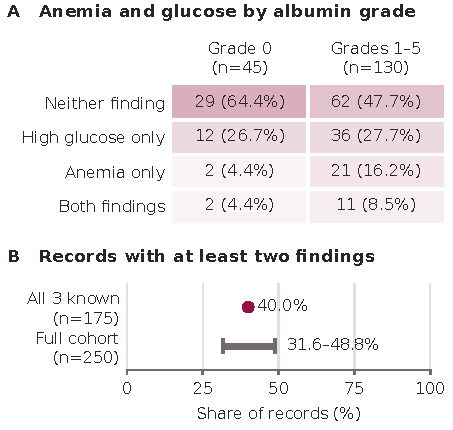
\includegraphics[width=\linewidth]{patient_overlap.pdf}\par
\vspace{5pt}
{\small Across all grades, \textbf{70 of 175 (40.0\%)} had at least two of these three findings (albumin grade~1 or higher, recorded anemia, and glucose at least 200~mg/dL). In all 250 records, the count ranged from 79 to 122 when missing results were counted first as absent, then as present. The line in panel B shows these bounds.\par}
\vfill
\casenote{BACK TO CASE 43}{Among the 45 grade-0 records, 16 had anemia, high glucose or both. Only two had \textbf{both}. Case 43 was one of them. Alongside grade 0 and creatinine of 1.0~mg/dL, the record showed hemoglobin of 9.7, a positive anemia flag and glucose of 204~mg/dL.}
\vspace{9pt}
{\color{muted}\hrule height0.3pt}\vspace{4pt}
{\footnotesize\raggedright\textbf{Data.} Rubini et al.\ (2015), \href{https://doi.org/10.24432/C5G020}{UCI Chronic Kidney Disease}.
\textbf{Clinical context.} NIDDK on \href{https://www.niddk.nih.gov/health-information/kidney-disease/chronic-kidney-disease-ckd/tests-diagnosis}{kidney tests}, \href{https://www.niddk.nih.gov/health-information/kidney-disease/anemia}{anemia in CKD}, \href{https://www.niddk.nih.gov/health-information/diabetes/overview/preventing-problems/diabetic-kidney-disease}{diabetes and kidney health} and \href{https://www.niddk.nih.gov/health-information/diabetes/overview/tests-diagnosis}{diabetes testing}.
\textbf{Analysis and figures.} Kassis et al.\ (2026), \href{https://doi.org/10.48550/arXiv.2609.00065}{Scientific Agent Skills}.\par}
\end{document}



